\documentclass[tikz,border=6pt]{standalone}
\usepackage{pgfplots}
\pgfplotsset{compat=1.18}
\usepgfplotslibrary{colormaps}
\usetikzlibrary{arrows, arrows.meta, calc}
\usetikzlibrary{decorations.markings}


\usepackage{amssymb,amsmath,mathtools}

\usepackage[T1]{fontenc}
\usepackage[utf8]{inputenc}
\usepackage{newpxtext,newpxmath}
\usepackage{sectsty}

\renewcommand{\Re}{\operatorname{\mathrm{Re}}}
\renewcommand{\Im}{\operatorname{\mathrm{Im}}}

\begin{document}
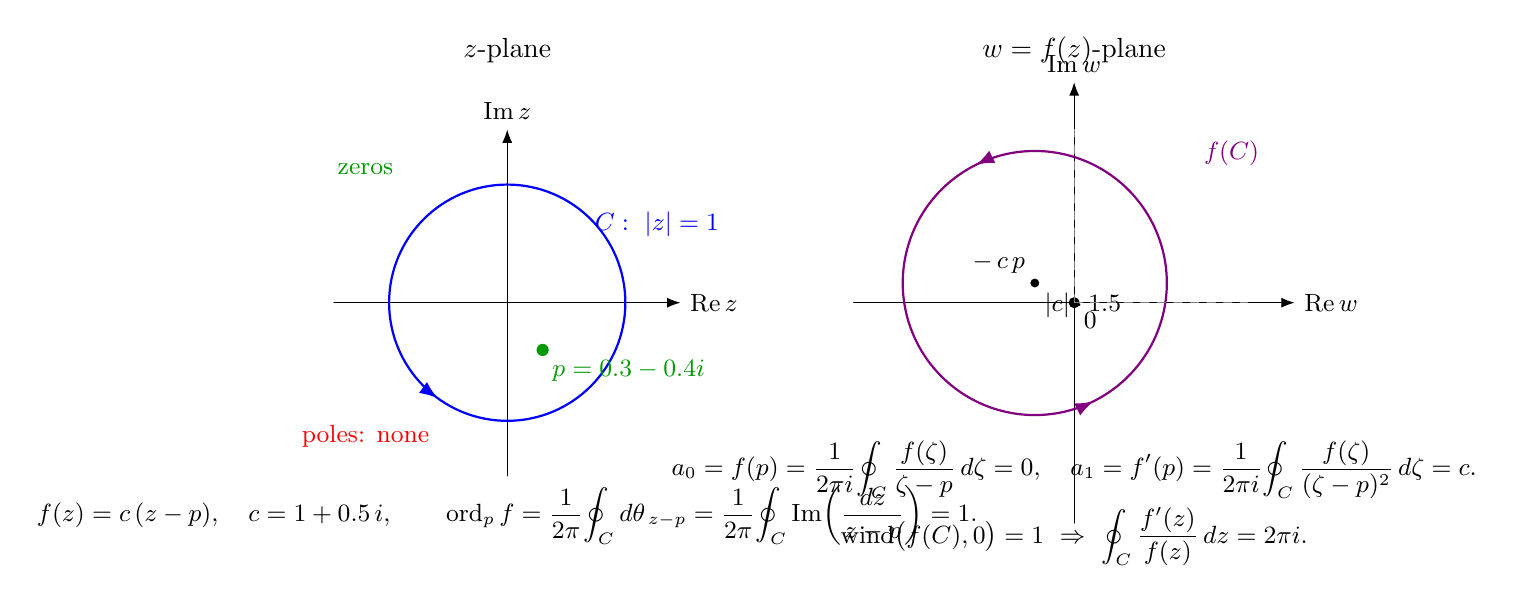
\begin{tikzpicture}[>=Latex, line cap=round, line join=round, font=\small]

%========================
% Left: z-plane
%========================
\begin{scope}[shift={(0,0)}]
	\node[font=\normalsize] at (0,3.2) {$z$-plane};
	% axes
	\draw[->] (-2.2,0)--(2.2,0) node[right] {$\Re z$};
	\draw[->] (0,-2.2)--(0,2.2) node[above] {$\Im z$};
	
	% unit circle C (positively oriented) -- radius 1.5 for visibility
	\draw[blue,thick,postaction={decorate},
	decoration={markings, mark=at position 0.65 with {\arrow{>}}}]
	(0,0) circle (1.5);
	\node[blue] at (1.9,1.0) {$C:\ |z|=1$};
	
	% zero at p (concrete choice inside C)
	\fill[green!60!black] (0.45,-0.6) circle(2.2pt) node[below right] {$p=0.3-0.4i$};
	\node[green!60!black] at (-1.8,1.7) {zeros};
	\node[red] at (-1.8,-1.7) {poles: none};
	
	% function label + order via winding form
	\node[align=left] at (0,-2.7) {$\displaystyle
		f(z)=c\,(z-p),\quad c=1+0.5\,i,\qquad
		\operatorname{ord}_{p} f
		=\frac{1}{2\pi}\!\oint_C d\theta_{\,z-p}
		=\frac{1}{2\pi}\!\oint_C \operatorname{Im}\!\left(\frac{dz}{z-p}\right)=1.$};
\end{scope}

%========================
% Right: w-plane = f(z)-plane
%========================
\begin{scope}[shift={(7.2,0)}]
	\node[font=\normalsize] at (0,3.2) {$w=f(z)$-plane};
	% axes
	\draw[->] (-2.8,0)--(2.8,0) node[right] {$\Re w$};
	\draw[->] (0,-2.8)--(0,2.8) node[above] {$\Im w$};
	
	% origin
	\fill (0,0) circle(2pt) node[below right] {$0$};
	
	% Parameters (hard-coded):
	% c = a+ib = 1 + 0.5i,  p = 0.3 - 0.4i
	% cp = c*p = (1+0.5i)(0.3-0.4i) = 0.5 - 0.25 i
	% So center of image circle is -cp = (-0.5, +0.25)
	% Image of C (radius 1.5) has radius |c|*1.5 with |c|=sqrt(1^2+0.5^2)=~1.118...
	% Param: z = 1.5 e^{it}  ->  w = c z - c p
	% Re w = 1.5*(a cos t - b sin t) - Re(cp)
	% Im w = 1.5*(a sin t + b cos t) - Im(cp)
	\draw[violet,thick,
	postaction={decorate},
	decoration={markings,
		mark=at position 0.25 with {\arrow{>}},
		mark=at position 0.75 with {\arrow{>}}}]
	plot[domain=0:6.283, samples=520]
	({ 1.5*(1.0*cos(\x r) - 0.5*sin(\x r)) - 0.5 },
	{ 1.5*(1.0*sin(\x r) + 0.5*cos(\x r)) + 0.25 });
	\node[violet] at (2.0,1.9) {$f(C)$};
	
	% mark the center of the image circle (-cp) and annotate |c|
	\fill[black] (-0.5,0.25) circle (1.6pt);
	\node[black,above left] at (-0.5,0.25) {$-\,c\,p$};
	\node[black,below right] at (-0.5,0.25) {$|c|\cdot 1.5$};
	
	% dashed rays to visualize winding (still +1)
	\draw[gray,dashed] (0,0) -- (2.2,0);
	\draw[gray,dashed] (0,0) -- (0,2.2);
	
	% annotation: Taylor coefficients at z_0=p via Cauchy integrals
	\node[align=center] at (0,-2.55)
	{$\displaystyle
		a_0=f(p)=\frac{1}{2\pi i}\!\oint_C \frac{f(\zeta)}{\zeta-p}\,d\zeta=0,\quad
		a_1=f'(p)=\frac{1}{2\pi i}\!\oint_C \frac{f(\zeta)}{(\zeta-p)^2}\,d\zeta=c.$\\[2pt]
		$\mathrm{wind}\big(f(C),0\big)=1 \ \Rightarrow\ \displaystyle \oint_C \frac{f'(z)}{f(z)}\,dz=2\pi i.$};
\end{scope}

\end{tikzpicture}
\end{document}